\chapter{Supervised Progressive Autonomous Robot Competencies}\label{chap:sparc}

\begin{framed}
	\textbf{Key points:}
	
	\begin{itemize}
		\item Novel interaction framework to teach robots how to interact while interacting
		\item Provide the human teacher control on the robot actions and the robot learns from the supervision
		\item Teacher provide feedback on intention rather than action
		\item The robot behaviour (under supervision) can be assumed to be optimal
		\item Reduce workload on the teacher over time as the robot learns
	\end{itemize}
\end{framed}

Parts of the work presented in this chapter have been published in \cite{senft2015sparc} and \cite{senft2017supervised}. The final publications are available from Springer and Elsevier via \url{http://dx.doi.org/10.1007/978-3-319-25554-5_60} and \url{https://doi.org/10.1016/j.patrec.2017.03.015}.

\newpage

\section{Principles}

As presented in Chapter \ref{chap:background}, robots would profit from being able to learn from humans how to interact with other humans. Using \gls{iml} to achieve this transfer of social and task knowledge from the human domain-expert to the robot would result in a faster approach than slow iterative update of behaviour by engineering an action policy or learning by trials and errors as with \gls{rl}.

However, as stated in that chapter, no current system provide the teacher with enough control over the robot action to ensure that the first principle presented in subsection \ref{ssec:back_constraints} (``Only execute appropriate actions.'') is validated. Techniques relying solely on feedback cannot prevent the robot to execute an incorrect action, but only reward negatively incorrect actions after their execution \citep{senft2017supervised}

In order to provide a robot with an appropriate action policy, adaptable to different users and requiring a low workload on the teacher or supervisor, we introduce the \acrfull{sparc} framework of interaction to allow end-users to safely teach a robot an action policy in \cite{senft2015sparc}.

\gls{sparc} defines an interaction between a learner and a teacher following these principles:
\begin{itemize}
	\item The learner has access to a representation of the state and a set of actions
	\item The teacher can select actions for the robot to do.
	\item The learner can propose actions to the teacher
	\item The teacher can enforce or cancel actions proposed by the learner, an actions non evaluate will be executed after a small delay
	\item The learner improves its action policy using the teacher's commands and feedback on propositions
\end{itemize} 
    
This way of keeping a human in the loop and in control of the robot's actions is equivalent to level 6 on the Sheridan scale of autonomy: "A computer selects action, informs human in plenty of time to stop it" \citep{sheridan1978human}. In addition, a learning algorithm improve the correctness of suggested actions decreasing the probability of requiring the teacher to correct actions or having to select new actions. Additionally, keeping the human in the loop allows them to provide additional information to the algorithm to speed up the learning and the control of the human over the robot actions ensures that every action executed by the robot is appropriate to the current state and simplify the learning algorithm too.

This approach is similar to predictive texting as seen on phone nowadays. The user can select the words proposed by the algorithms, or write their own, and the algorithm learns the user's preferences and habits and aims to suggest word more and more appropriate to the user. However, \gls{sparc} is aimed to be used is more complex, interactive environments, reacting to the user's selection and to the world surrounding the agent.

%TODO: add difference with active learning, the agent cannot decide which sample it will evaluate and these are provided by the environment
\section{Goal}

The goal of \gls{sparc} is to achieve quickly an autonomous appropriate action policy by interacting, without requiring constant action from a human whilst ensuring that the action policy is appropriate. 

Figure \ref{fig:concept} presents an idealist comparison of the expected workload, performance and autonomy of three methods: autonomous learning (such as \gls{rl} \cite{sutton1998reinforcement}), feedback based teaching (such as TAMER \cite{knox2009interactively}) and \gls{sparc}. Unlike other methods, by following the principles presented in the previous section, \gls{sparc} is expected to maintain a constant high performance even during early stages of learning, and to see a decrease of workload on human supervisor as the agent improve its action policy using machine learning and the suggestions become more accurate.

%TODO: could add woz
\begin{figure}[ht]
	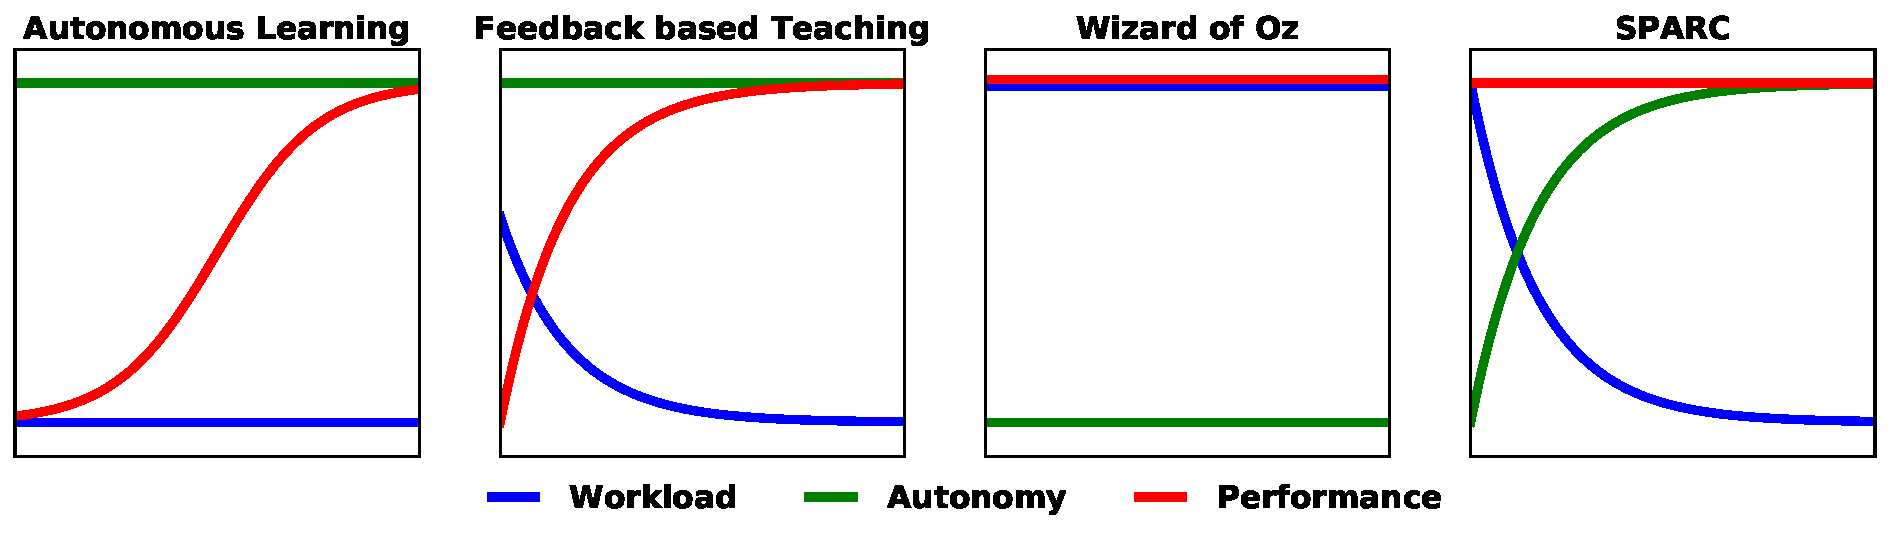
\includegraphics[width=.8\linewidth]{concept.pdf}
	\centering
	\caption{Idealistic comparison between autonomous learning, feedback base teaching and \gls{sparc}.}
	\label{fig:concept}
\end{figure}

Once the behaviour is deemed appropriate enough by the teacher, the agent can be deployed to interact autonomously in the real world if this is the desired output. Alternatively, in context where a human expert cannot be removed from the control loop, such as \acrlong{rat}, the supervisor can stay in control of the robot actions in a supervised autonomous way (level 6 of Sheridan) and only intervene when the agent is about to do an error. This approach is similar to safety drivers behind autonomous vehicles but with more information about what the car would be about to do. 

\section{Frame}

Similar to other application of \gls{iml}, SPARC requires the presence of a teacher. As such, the type of interaction possible would be either: dyadic interaction (Supervisor-Robot-Supervisor or Supervisor-Robot-Environment), such as  robot at home learning from its user how to support them better or triadic interaction (Supervisor-Robot-Human partner), such as a teacher teaching a robot tutor how to support child learning (as implemented in Chapter \ref{chap:education})

However, unlike other \gls{iml} approaches, the requirement of a human in the action selection loop limits the timescale of interaction. As the human has to be provided with few seconds to react to the proposition, the rate of actions has to be .5Hz or below. However, this can be mitigated by using higher level actions and this has the advantage to ensure that only correct actions will be executed without requiring the human to select them all.

\gls{sparc} presents many similarities with \acrlong{lfd} as it uses human demonstration of action to learn. However, most of the applications of \gls{lfd} \citep{argall2009survey,billard2008robot} are focused on learning a manipulation skill in a mostly deterministic environment. \gls{lfd} has seldom been used to teach an action policy to interact with humans \cite{liu2014train,sequeira2016discovering} and never in an online fashion.

\section{Interaction with Machine Learning Algorithms}

Supervised Learning

Reinforcement learning 

Other type of learning (ex: instance based learning)

\section{Summary}
    
    

